\documentclass[10pt,aspectratio=43,mathserif]{beamer}		
%设置为 Beamer 文档类型,设置字体为 10pt,长宽比为16:9,数学字体为 serif 风格

%%%%-----导入宏包-----%%%%
\usepackage{jnubeamer}
\usepackage{xeCJK}
\usepackage{amsmath,amsfonts,amssymb,bm}
\usepackage{color}
\usepackage[version=4]{mhchem}
\usepackage{graphicx,hyperref,url}	
\renewcommand{\today}{\number\year 年\number\month 月\number\day 日}
%%%%%%%%%%%%%%%%%%


%%%%-----设置字体-----%%%%
%Windows和Mac OS下都可用
\setsansfont{arial.ttf}
%\setsansfont{Times New Roman}

%设置 Beamer 主题
\beamertemplateballitem
\definecolor{beamer@blendedblue}{rgb}{0.153,0.365,0.514}
\renewcommand{\thefootnote}{\fnsymbol{footnote}}
\AtBeginSection[]
{
  \begin{frame}<beamer>
    \frametitle{\textbf{目录}}
    \textbf{\tableofcontents[currentsection]}
  \end{frame}
}

%%%%----首页信息设置----%%%%
\title[含硒表面活性剂囊泡的构筑与性质研究]{\fontsize{13pt}{18pt}\selectfont {含硒表面活性剂囊泡的构筑与性质研究}}
\subtitle{\fontsize{9pt}{14pt}\selectfont \textbf{毕业论文答辩}}			

\author[陈育明]{\makebox[4em][s]{答辩人}:陈育明\\\medskip
指导教师:刘雪锋
}
%    陈育明  \\\medskip
%    {\small {应用化学1502班}}
\institute[SCME]{
  化学与材料工程学院\\
  江南大学}

\date[2019年6月8日]{
 2019年6月8日}

\begin{document}

\begin{frame}
\titlepage
\end{frame}				%生成标题页



\section*{目录}

		\begin{frame}
		\frametitle{目录}
		\tableofcontents
		\end{frame}				%生成提纲页

\section{引言}

    \begin{frame}
    \frametitle{引言}
    \begin{block}{what}
        \begin{itemize}
        \item what ,what;
        \item what:what,what;
        \end{itemize}
    \end{block}
    \begin{block}{what:what\footnotemark[1]}
        \begin{itemize}
        \item what、what E;
        \item what,what. 
        \end{itemize}
    \end{block}
    \footnotetext[1]{doi:10.1038/s41467-017-00419-5}
    \end{frame}

\section[制备]{含硒表活}

 \begin{frame}
\frametitle{制备}
    \begin{figure}[htbp]
    \centering
    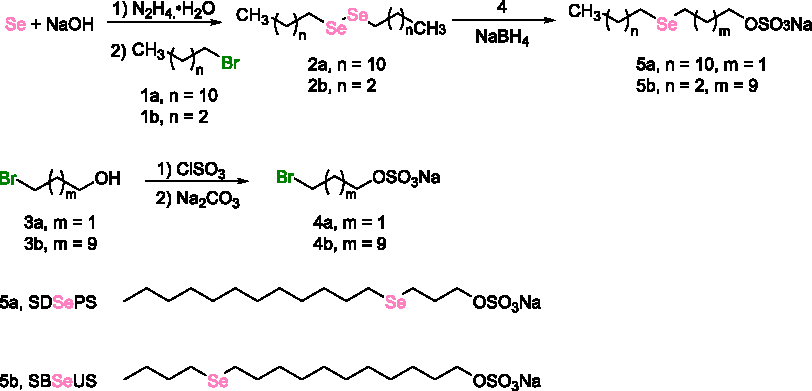
\includegraphics[width=0.86\textwidth]{figure/scheme-synthesis.pdf}\\
    \caption{含硒表面活性剂的合成路线}\label{fig:synthesis}
\end{figure}
\end{frame}

\section{表征}
\begin{frame}{SDSePS \ce{^1H NMR}}
    \begin{figure}[htbp]
        \centering
        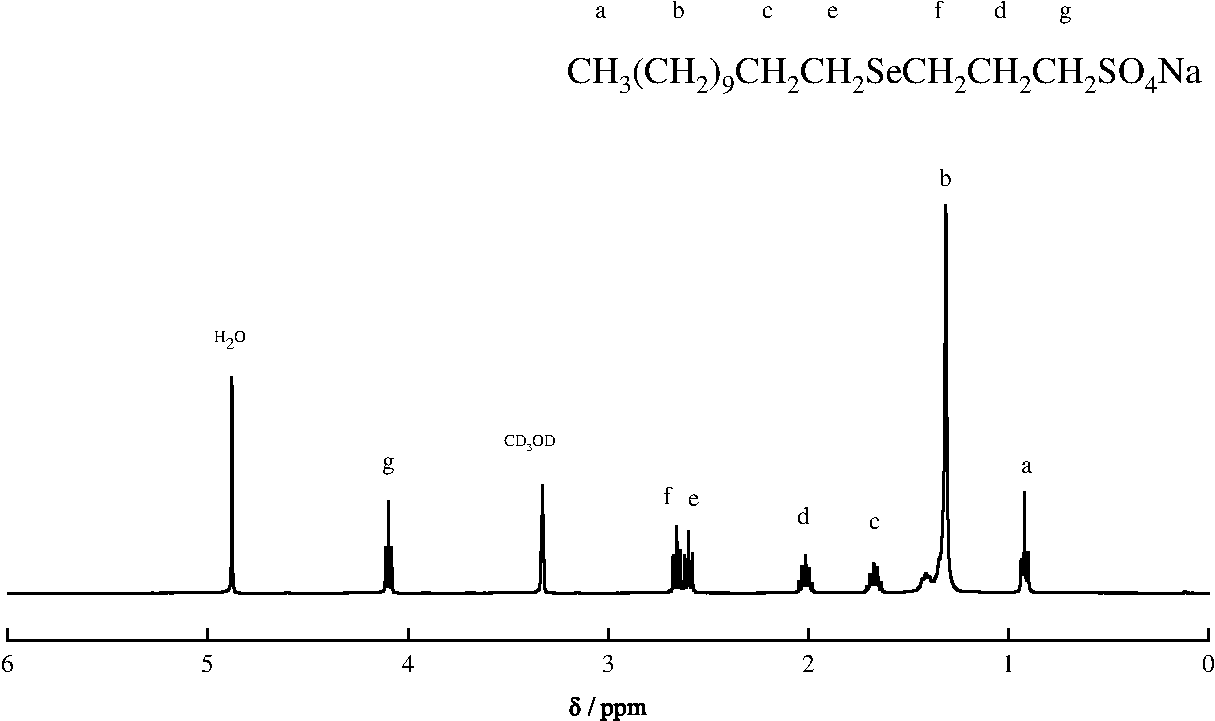
\includegraphics[width=.85\textwidth]{figure/SDSePS-nmr.pdf}\\
        \caption{SDSePS的核磁氢谱}\label{fig:SDSePS-nmr}
    \end{figure}
%    {\footnotesize
%    \ce{^1H} NMR (400 MHz, \ce{CD3OD}, 图\ref{fig:SDSePS-nmr}) δ 0.92 (t, \textit{J}=8.0 Hz, 3H), 1.31-1.41 (overlap, 18H), 
%    1.67 (m, 2H), 2.01 (m, 2H), 2.60 (t, \textit{J}=8.0 Hz, 2H), 2.66 (t, \textit{J}=8.0 Hz, 2H),  4.10 (t, \textit{J}=6.0 Hz, 2H).
%}
\end{frame}

\begin{frame}
\frametitle{耐盐性}
\begin{columns}[c]
\column{0.38\textwidth}
%\begin{figure}[!t]
%    \centering
%    \includegraphics[width=.99\textwidth]{figures/spf-eggs.jpg}
%    \caption{SPF(无特定病原体)鸡蛋}
%\end{figure}
\column{0.62\textwidth}
\begin{itemize}
    \item 工艺步骤:对SPF鸡蛋接种、培育、收集(病毒)原液、灭活、超滤纯化;
    \item 特点:安全有效、工艺成熟(发端自20世纪40年代);
    \item 不足:生产周期稍长(5-6月),应对全球流感稍显乏力,存在鸡蛋过敏症状.
\end{itemize}
\end{columns}
\end{frame}

\begin{frame}{耐盐性}
    \begin{columns}[c]
    \column{0.5\textwidth}
        \begin{figure}[htbp]
            \centering
            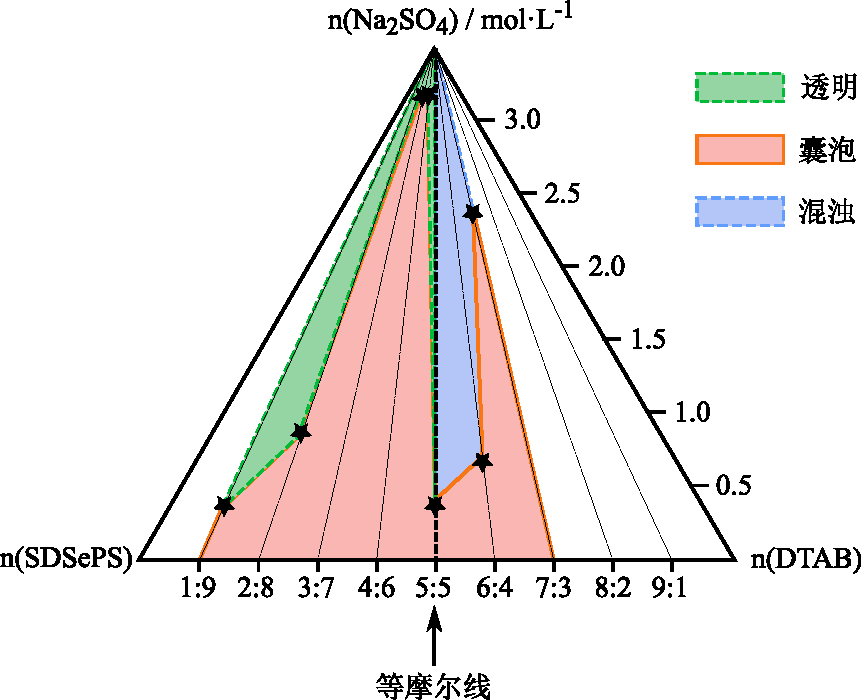
\includegraphics[width=0.92\linewidth]{figure/SDSePS-salt.pdf}\\
            \caption{SBSeUS/DTAB囊泡示意图}\label{fig:SDSePS-salt}
        \end{figure}
    
    \column{0.5\textwidth}
        \begin{figure}[htbp]
            \centering
            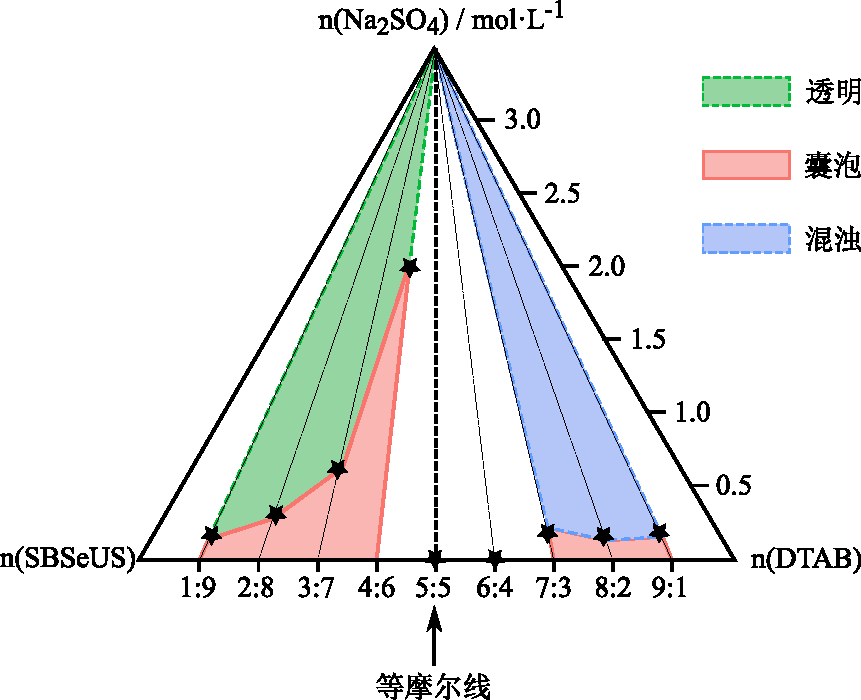
\includegraphics[width=0.92\linewidth]{figure/SBSeUS-salt.pdf}\\
            \caption{SBSeUS/DTAB囊泡示意图}\label{fig:SBSeUS-salt}
        \end{figure}
    
    \end{columns}
\end{frame}

    \begin{frame}
    \frametitle{\textbf{青霉素发酵工艺}}
        \begin{block}{种子的培养}
            种子的培养是发酵过程中十分关键的步骤,主要作用是通过孢子的不断繁殖,从而得到充足的霉菌菌丝,优良的种子移入发酵罐,
            能够快速适应新的培养环境,种子的制备一般是先进行摇瓶培养,随后在种子罐中进行逐级扩大培养。
        \end{block}
    \end{frame}

       \begin{frame}
        \frametitle{食品工业}
        \begin{block}{开发功能性食品辅料}
            \begin{enumerate}
                \item 亚麻酸
                \item 新糖源
                \item 功能性油脂
            \end{enumerate}
        \end{block}
        \end{frame}

		\begin{frame}
		  \frametitle{微生物处理污水}
          \textbf{根据微生物的存在状态}
          \begin{columns}[c]
          \column{.45\textwidth}
    		  \begin{block}{活性污泥法}
                  应用最广泛;含溶解性有机物污水中连续鼓入空气形成活性污泥,微生物以有机物为食并将其分解;
              \end{block}
          \column{.45\textwidth}
              \begin{block}{生物膜}
                污水连续流经固体填料生成污泥状的生物膜,其上繁殖着大量微生物,与活性污泥作用相同.
              \end{block}
          \end{columns}
      
          \textbf{根据微生物需氧与否}
          \begin{columns}[c]
              \column{.45\textwidth}
              \begin{block}{\textbf{厌氧生物处理}}
                  利用兼性厌氧菌和专性厌氧菌在无氧条件下降解有机污染物的处理技术;
              \end{block}
              \column{.45\textwidth}
              \begin{block}{\textbf{好氧生物处理}}
                  利用好氧微生物(包括兼性微生物)在有氧气存在的条件下进行生物代谢以降解有机物.
              \end{block}
          \end{columns}
		\end{frame}
%======封底============================================================
\section*{}
            \begin{frame}

                \begin{center}
                    \begin{minipage}{1\textwidth}
                        \setbeamercolor{mybox}{fg=white, bg=beamer@blendedblue}
                        \begin{beamercolorbox}[wd=0.70\textwidth, rounded=true, shadow=true]{mybox}
                        \LARGE \centering Thanks for Listening.
                        \end{beamercolorbox}
                    \end{minipage}
                \end{center}

%                \begin{figure}[!t]
%                    \centering
%                    \includegraphics[width=.8\textwidth]{figures/figure5.png}
%                    \label{figure4_ad}
%                \end{figure}
            \end{frame}
\end{document} 